% vim: set spell spelllang=es syntax=tex :

\section{Metodología experimental}

Como se menciono con anterioridad, para comprobar el funcionamiento del nuevo
framework se procesaron los vídeos de resolución 800x600 y 1280x720, en una
computadora con un procesador Intel Xeon E5-2630. Este es un procesador de 6
núcleos, cada uno de dos subprocesos simultáneos a través de la técnica de
\emph{simultaneus multithreading} y con un reloj de 2,30GHz. El equipo cuenta
ademas con 16GiB de memoria RAM, 15MiB de memoria cache L3, 256KiB de cache L2,
32Kib de cache L1 para datos, y 32 KiB de cache L1 para instrucciones. El vídeo
de 800x600 píxeles de resolución permitirá comprobar el rendimiento del sistema
con la carga equivalente a un vídeo de una cancha de tamaño doble, mientras que
el vídeo de 1280x720 píxeles de resolución permitirá comprobar la adaptabilidad
del sistema a cargas mayores.

\begin{figure}[!ht]

	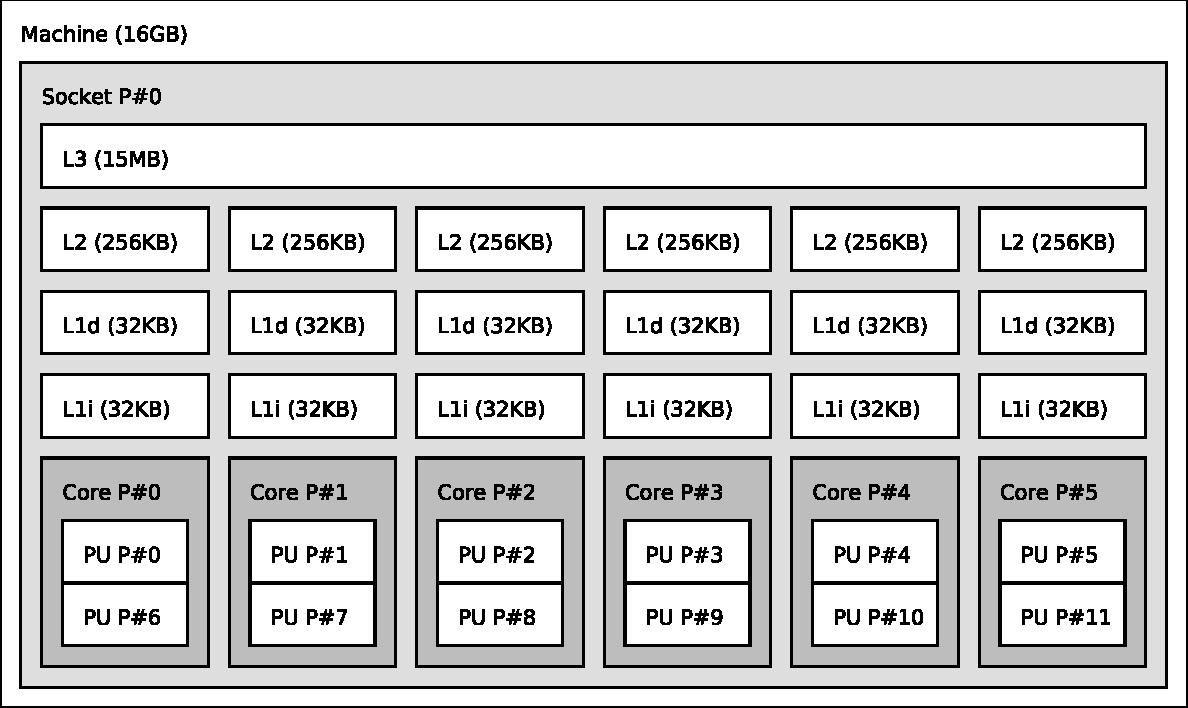
\includegraphics[width=\textwidth]{img/topo.pdf}
	\caption{Arquitectura de la maquina de pruebas.}

\end{figure}

Se realizaron pruebas con cada vídeo, variando la cantidad de partes en las que
fueron divididos los cuadros de 1 a 24, y la cantidad de hilos de búsqueda entre
1 y 12. Cada prueba se ejecuto dos veces, la primera buscando el mínimo de la
cantidad máxima de cuadros por segundo que soporta el sistema bajo cada
configuración. En la segunda se limito la cantidad de cuadros por segundo de
cada configuración, según lo encontrado en la primer prueba, y se registró el
tiempo de procesamiento de los cuadros máximo para cada de estas. Cada prueba
consto de 10 ejecuciones distintas de las que solo se registró el peor valor
obtenido.

Dada la gran cantidad de ejecuciones se busco el tiempo mínimo necesario para
que estas fueran representativas de una ejecución prolongada. Se realizaron 3
ejecuciones con 11 hilos y 12 fragmentos, durante 11 minutos. El primer minuto
no se contabilizo con el fin de permitir que la ejecución se estabilizara.
Estas se compararon con ejecuciones bajo la misma configuración, pero ejecutando
de 10 a 20 segundos, y contabilizando solo los últimos 10. Con esta prueba se
pudo comprobar que las pruebas de 16 segundos son representativas de ejecuciones
mas largas.

Durante el desarrollo de la aplicación se probaron tres distintas
implementaciones. En la primera implementación, el framework ejecutaba las
distintas pilas de plugins en tareas separadas. En la segunda implementación el
framework fue modificado para que una sola tarea ejecutara todas las pilas de
plugins sobre un mismo fragmento. Para la tercera implementación se trabajo
sobre el mismo framework que la segunda, pero se unieron las pilas de búsquedas
de robots y la de búsqueda de pelota. De estas, la última fue la que produjo
resultados mas satisfactorios, por lo que sera sobre los resultados de esta que
trabajaremos a continuación.

\section{Resultados}

Como se pueden ver en las figuras \ref{800fps} y \ref{1280fps}, se cumplió
satisfactoriamente con el objetivo crear un sistema capas de procesar un vídeo
de 800x600 píxeles a 60 cuadros por segundo, llegando a triplicar la cantidad de
cuadros por segundos buscados. También se logro superar esta taza en el vídeo de
1280x720 píxeles de resolución, indicando que el sistema podría ser usando bajo
estas condiciones.

\begin{figure}[!h]

	\includegraphics[width=\textwidth]{img/800x600_fps.pdf}
	\caption{}
	\label{800fps}

\end{figure}

\begin{figure}[!h]

	\includegraphics[width=\textwidth]{img/1280x720_fps.pdf}
	\caption{}
	\label{1280fps}

\end{figure}

En las figuras \ref{800fps} y \ref{1280fps} se pueden observar dos patrones que
ocurren en ambos vídeos y cuyas causas pueden ser no inmediatamente obvias. El
primero es que si los cuadros se dividen en 7, 11, 17, 19 y 23 fragmentos, se
produce una notable reducción en la cantidad de cuadros por segundo con respecto
a las divisiones adyacentes. El segundo patrón que se puede observar es una
reducción en la cantidad de cuadros por segundo cuando la cantidad de fragmentos
es reducida y la cantidad de hilos de búsqueda alta.

Dado que el orden de ejecución de la pila de plugins es del orden de la suma del
área de los fragmentos, es de esperar que a mayor área total, menor sea la
cantidad de cuadros por segundo, por lo cual mayor cantidad de fragmentos,
implicaría una reducción en la cantidad de cuadros procesados. Pero al mismo
tiempo, mayor cantidad de fragmentos permite aprovechar el paralelismo de mejor
manera. Sin embargo, la relación entre cantidad de fragmentos y el área es
irregular. Si se divide el cuadro en un número primo de fragmentos, el área
total se incrementa de forma significativa con respecto a los valores
circundantes. En la figura \ref{primosArea} se muestra la fluctuación del área
para cada cantidad de particiones desde 1 hasta 100 para un vídeo de 1280x720
píxeles de resolución, resaltando el crecimiento para valores primos y para los
valores inmediatamente inferiores y superiores. Como puede observarse, a partir
de 7 fragmentos el área total se incrementa de forma significativa cuando el
número es primo con respecto a los valores cercanos no primos.

\begin{figure}[!h]

	\includegraphics[width=\textwidth]{img/primos_area.pdf}
	\caption{}
	\label{primosArea}

\end{figure}

Para comprobar como esta variación de volumen de datos afecta la cantidad de
cuadros por segundo procesados, se realizaron nuevas pruebas sobre el vídeo de
1280x720 píxeles de resolución, con 11 hilos de búsqueda y variando la cantidad
de fragmentos entre los números primos mayores a 24 y menores a 100, y sus
inmediatos superior e inferior. Los valores para números primos e inmediatos
inferiores a 24 fueron tomados de los experimentos anteriores. Los resultados
pueden ser observados en la figura \ref{primosFPS}.

\begin{figure}[!h]

	\includegraphics[width=\textwidth]{img/primos_fps.pdf}
	\caption{}
	\label{primosFPS}

\end{figure}

Como se puede observar en la figura, para una cantidad de fragmentos menor a 7,
el perjuicio por aumento en el área es menor que el beneficio aportado por el
incremento en el paralelismo. Si se observa la figura \ref{primosArea}, dividir
el cuadro en 7 fragmentos resulta en el primer incremento notable de área con
respecto tanto a un fragmento menos como un fragmento más. También se pueden
apreciar que los incrementos repentinos en el área total coinciden con
disminuciones repentinas en los cuadros por segundo procesados.

TODO: ¿Falta aclarar algo al respecto?

Para encontrar las cusas del segundo patrón (la reducción en cuadros por
segundos procesados cuando la cantidad de hilos de búsqueda es alta, y la
cantidad de fragmentos baja) se realizo una búsqueda manual del fragmento de
código donde se producía el retardo. Finalmente se pudo comprobar que la causa
principal de este retardo se produce en una función de una librería externa.
Analizando el código de esta se encontró que la fuente principal del retardo se
trata de un segmento de código que accede a todos los píxeles de una imagen
auxiliar y lo colorea de negro. Por cada fragmento se crea una de estas imágenes
auxiliares y su tamaño es igual al tamaño del fragmentos del cuadro.

Dado que la causa del retardo se trata de una operación intensiva en memoria, y
que su efecto se observa cuando el tamaño del fragmentos (y por lo tanto de la
imagen sobre la que se realiza la operación) es grande, se propuso la hipótesis
de que el retardo se produce dado que los hilos compiten por el espacio de
cache.

Para comprobar que esta explicación es correcta se ejecuto el programa
procesando el vídeo de 1280x720 píxeles de resolución, donde cada curva muestra
los resultados de dividir la imagen en 1, 2, 6 o 12 fragmentos, variando la
cantidad de hilos de búsqueda de 1 a 11 y midiendo los fallos de cache. Los
resultados pueden ser observados en la figura \ref{cacheFallos}.

\begin{figure}[!h]

	\includegraphics[width=\textwidth]{img/cache_fallos.pdf}
	\caption{}
	\label{cacheFallos}

\end{figure}

Si se observa detenidamente cada curva de la figura, se pueden distinguir una
etapa de crecimiento acelerado, seguido de una etapa de crecimiento mas gradual.
En los casos de 1 y 2 fragmentos, el cambio es pronunciado, y se puede verificar
en la figura \ref{1280fps} que es justamente bajo esta configuración donde, dado
ese numero de fragmentos, agregar un hilo de búsqueda más reduce la cantidad de
cuadros procesados.

Finalmente, en las figuras \ref{800turnArround} y \ref{1280turnArround} se
pueden observar los tiempos máximos de espera de procesamiento de los cuadros,
para los vídeos de 800x600 y 1280x720 píxeles de resolución limitando los
cuadros por segundo generados al máximo encontrado en los experimentos
anteriores.

\begin{figure}[!h]

	\includegraphics[width=\textwidth]{img/800x600_turnArround.pdf}
	\caption{}
	\label{800turnArround}

\end{figure}


\begin{figure}[!h]

	\includegraphics[width=\textwidth]{img/1280x720_turnArround.pdf}
	\caption{}
	\label{1280turnArround}

\end{figure}

Estos dos últimas figuras nos permiten apreciar que no siempre una mayor
cantidad de cuadros por segundos procesados implicara el tiempo de retardo
mínimo. Dependiendo de si se desea minimizar el retardo de procesamiento de los
cuadros, maximizar la cantidad de cuadros procesados, o encontrar un balance
especifico, se deberá elegir una cantidad de fragmentos y procesadores
apropiada. Por ejemplo, en el caso del vídeo de 1280x720 píxeles de resolución,
dividir la imagen en 21 fragmentos y utilizar 11 utilizar permite procesar 94
cuadros por segundo en el equipo de prueba, sin embargo el retardo es de $0.09$
segundos. Si el cuadro se divide en 15 fragmentos y se utilizan 11 hilos de
búsqueda, la cantidad de cuadros por segundo procesados se cae a 90, pero el
retardo se reduce a $0.05$ segundos.
